\documentclass{../../oss-handout}
\usepackage{tikz}
\usepackage{newtxtext,newtxmath}
\usepackage{enumitem}
\usepackage{graphics}
\usepackage[ISO]{diffcoeff}

\setlength{\parindent}{0pt}
\setlength{\parskip}{2pt}
\setlength{\headheight}{26pt}

\tikzset{
	>=latex,
}

\usetikzlibrary{decorations.pathmorphing,patterns}

\tikzstyle{springy}=[decorate,decoration={
    coil,
    segment length=4pt,
    aspect=.6,
    amplitude=4pt,
    pre=lineto,
    pre length=1mm,
    post=lineto,
    post length=1mm},thick]
\tikzstyle{mass}=[draw,minimum size=.6cm,fill=cyan!20,thick]

\newcommand{\pic}[2]{\includegraphics[width=#1\textwidth]{#2}}

% Set the page style for the document
\pagestyle{plain}

% Course & handout information
\renewcommand{\institution}{Meritus Academy}
\renewcommand{\coursetitle}{Physics 11}
\renewcommand{\term}{Updated for Fall 2022}

\tikzstyle{springy}=[decorate,decoration={
    coil,
    segment length=4pt,
    aspect=.7,
    amplitude=4pt,
    pre=lineto,
    pre length=1mm,
    post=lineto,
    post length=1mm},thick]
\tikzstyle{mass}=[draw,minimum size=.6cm,fill=cyan!20,thick]

\title{Additional Notes for Teachers on Sound Waves}
\author{Tim}
\date{\today}

\begin{document}
\thispagestyle{title}
\gentitle

Here are some additional background information for teachers and students. The
material on this document should not be part of the class, as this is clearly
well beyond the realm of Grade 11 Physics. However, this information may be
useful in guiding you when confronted with questions from students, which can
be quite challenging. This document is constantly being updated, but should not
be sent to students.
\begin{itemize}[leftmargin=10pt]
\item\textbf{Speed of Sound:} The equations for speed of sound sometimes
  generate a lot of discussion in class\footnote{it had, at times, dominated
  in-class discussions, but at other times, there are no discussions at all},
  particularly with how the speed varies in different media (gases, solids,
  liquids). The speed of any wave (mechanical or electromagnetic) is contained
  the 2nd-order wave equation. In one dimension:
  \begin{equation}
    \diffp[2]ut=\varv^2\diffp[2]ux
  \end{equation}
  This wave equation itself can be derived through first principle (i.e.\
  second law of motion), by modelling the medium as masses connected by
  massless springs, with stiffness $k$, as we have shown in a diagram in the
  previous class. The distance between the massses is $h$. The schemetics is
  shown in Figure~\ref{medium}.
  \begin{figure}[ht]
    \centering
    \begin{tikzpicture}[scale=1.2]
      \node[mass] (m1) at (0,0) {$m$};
      \node[mass] (m2) at (2,0) {$m$};
      \node[mass] (m3) at (4,0) {$m$};
      \node[mass] (m4) at (6,0) {$m$};
      \node[mass] (mx) at (12,0) {$m$};
      \draw[springy] (m1)--(m2) node[midway,above=2.5]{$k$};
      \draw[springy] (m2)--(m3) node[midway,above=2.5]{$k$};
      \draw[springy] (m3)--(m4) node[midway,above=2.5]{$k$};
      \draw[springy] (m4)--(7.6,0) node[midway,above=2.5]{$k$};
      \draw[springy] (10.4,0)--(mx) node[midway,above=2.5]{$k$};
      \foreach \x in {8,8.25,...,10} \fill (\x,0) circle(.04);
      \draw[|<->|] (0,-.5)--(2,-.5) node[midway,fill=white]{$h$};
    \end{tikzpicture}
    \caption{Model of a medium for mechanical waves}
    \label{medium}
  \end{figure}
  
  This derivation is neither simple nor straightforward, and therefore not
  usually done even in undergrad or grad-level courses\footnote{Anecdotally, my
  own experience with this derivation is that it is too difficult for an
  undergraduate course, and too trivial for graduate students.}. From the
  second law of motion, we can show that the speed of an acoustic wave is
  determined by the ratio of the medium's elastic and inertial properties.
  \begin{equation}
    \varv=\sqrt{\frac{\text{elastic property}}{\text{inertial property}}}
    \label{elas-over-inertia}
  \end{equation}
  Therefore, the speed of sound in a fluid (i.e.\ liquid or gas) reduces to
  the equation given in class:
  \begin{equation}
    \varv_s=\sqrt{\frac K\rho}
  \end{equation}
  $K$ is the fluid's bulk modulus; it refers to the substance's resistance to
  compressive force, i.e.:
  \begin{equation*}
    K = -V\diff PV
  \end{equation*}
  For an ideal gas, the bulk modulus is simply $K=\gamma P$. By applying the
  ideal gas law, we get two additional expressions for the speed of sound in a
  gas:
  \begin{equation}
    \varv_s=\sqrt{\frac{\gamma P}\rho}=\sqrt{\frac{\gamma RT}M}
  \end{equation}
  where $R$ is the gas constant, $M$ is the molar mass of the gas, and $T$ is
  the thermodynamic/absolute temperature. The last expression is notable
  because it bears striking resemblance to the most probable, mean and
  root-mean-square speeds of a gas at temperature $T$. For solids, the equation
  for the speed of sound is
  \begin{equation}
    \varv_s=\sqrt{\frac E\rho}
  \end{equation}
  where $E$ is the Young's modulus of the solid, which relates a solid's strain
  ($\sigma$) under tensile stress ($\epsilon$):
  \begin{equation*}
    E=\frac\sigma\epsilon=\frac{F/A}{\dl l/l}
  \end{equation*}
  Based on the derivation of the wave equation, the fact that the speed of
  sound is fastest in solids, then in liquids, then solids is \emph{not}
  because the inter-molecular distance is shorter in solids than liquids and
  gases, as commonly asserted by many high-school physics
  teachers\footnote{Imaging what interviews look like!}. Helium gas is
  generally low in density, but the speed of sound is almost 3 times faster
  than in air. This is consistent with Eq.~\ref{elas-over-inertia}, but the
  ``common explanation'' fails to account for it.

\item\textbf{Decibel:} The most common answer when asked why the
  intensity/loudness of sound is expressed using a logarithmic scale is that
  logarithmic scales allow us to \emph{manage numbers that span many orders of
  magnitude}. I have found several references to this explanation while doing
  a quick search online. While this may be the case in general, the actual
  reason for using a logarithmic scale is more nuanced. In this case, the human
  brain perceives a ``doubling'' of loudness when the intensity is increased by
  approximately one order of magnitude. This is known as the
  \emph{Webner-Fechner law}, in a research area called psyphophysics, which has
  shown that the human perception of loudness of sound (or brightness of light)
  is proportional to a logarithm of the actual intensity measured by an
  accurate instrument.

\item\textbf{Bullet:} In the photo of the bullet, shown in Figure~\ref{bullet},
  there are three shocks that are clearly visible. The first one is just ahead
  of the leading edge of the fullet; the second is about $2/3$ of the way along
  the length of the bullet, where the bullet joins  the casing; the third is
  along the turbulent wake behind the bullet. The Mach angles are different,
  therefore the Mach numbers does, in fact, change as air flows around the
  bullet.
  \begin{figure}[ht]
    \centering
    \pic{.4}{../images/bullet2}
    \caption{Three shock waves around a bullet}
    \label{bullet}
  \end{figure}
  
\item\textbf{Shock tube:} The slide with the supersonic bullet made reference
  to a ``shock tube'' that generates the supersonic flow around the bullet. The
  experimental set up is actually quite simple. Air at two different pressures
  are separated by a membrane. At the time of the experiment, an explosive
  charge detonates the membrane, allowing a supersonic flow to be generated.
  \begin{figure}[ht]
    \centering
    \begin{tikzpicture}
      \draw[line width=3.5,magenta] (3,0)--(3,1);
      \draw[ultra thick] (10,0)--(0,0)--(0,1)--(10,1);
      \node at (1.5,.5){$P_\text{high}$};
      \node at (6.5,.5){$P_\text{atm}$};
    \end{tikzpicture}
    \caption{A basic shock tube.}
  \end{figure}
  
\item\textbf{Harmonic Frequencies:} The concept of harmonic frequencies is
  based on the Fourier series, in which any periodic function $f(x)$ with
  period $P$ can be written as a sum of sinusoidal functions, i.e.\
  \begin{displaymath}
    f(x)=\frac{a_0}2 + \sum_{k=1}^\infty 
    \left[
      a_k\sin\left(\frac{2\pi k}Px\right) +
      b_k\cos\left(\frac{2\pi k}Px\right)
    \right]
  \end{displaymath}
  If this shape represents a harmonic wave travelling through space with a
  wavelength $\lambda$, then the wave function $\Psi$ can be given by
  \begin{displaymath}
    \Psi(x,t)=\frac{a_0}2 + \sum_{k=1}^\infty
    \left[
      a_k\sin\left(\frac{2\pi k}\lambda x-k\omega t\right) +
      b_k\cos\left(\frac{2\pi k}\lambda x-k\omega t\right)
    \right]
  \end{displaymath}
  Either way, the frequency $k\omega$ and the wave number (spatial frequency)
  $nk$ are integer multiples of a fundamental frequency.
\end{itemize}
\end{document}
